\documentclass[10pt]{article}
%General Packages
\usepackage{multicol, enumerate, enumitem, hyperref, color, soul, setspace, parskip, fancyhdr}

%Math Packages
\usepackage{amssymb, amsthm, amsmath, bbm, latexsym, units, mathtools}

%All math in Display Style
\everymath{\displaystyle}

% Packages with additional options
%\usepackage[T1]{fontenc}
\usepackage[headsep=0.5cm,headheight=0cm, left=1 in,right= 1 in,top= 1 in,bottom= 1 in]{geometry}
\usepackage[usenames,dvipsnames]{xcolor}

% SageTeX
\usepackage{sagetex}

% Package to use the command below to create lines between items
\usepackage{dashrule}
\newcommand{\litem}[1]{\item#1\hspace*{-1cm}\rule{\textwidth}{0.4pt}}

\pagestyle{fancy}
	\lhead{Module 5 - Radical Equations}
	\chead{}
	%CHECK Version
	\rhead{Progress Exam 3}
	\lfoot{Spring 2019}
	\cfoot{}
	\rfoot{Make-Up Version}

\begin{document}
	\pagestyle{fancy}

\begin{sagesilent} 
load("../Code/generalPurposeMethods.sage")
load("../Code/keyGeneration.sage")
\end{sagesilent}

\begin{enumerate}
\setcounter{enumi}{20}

% Objective 1 - Identify the domain on which a radical function is not defined.
\begin{sagesilent}
moduleNumber = 5
version = "MU"
problemNumber = 21
load("../Code/radical/domainRadical.sage")
\end{sagesilent}

\litem{ \sage{displayStem} 

	$$ \sage{displayProblem} $$
	\begin{enumerate}[label=\Alph*.]
		\item $\sage{choices[0]}$ 
		\item $\sage{choices[1]}$ 
		\item $\sage{choices[2]}$ 
		\item $\sage{choices[3]}$ 
		\item $\sage{choices[4]}$ 
	\end{enumerate}	
\vspace*{-3mm}
}

% Objective 2 - Identify the graph of a radical function (graph to equation).
\begin{sagesilent}
problemNumber = 22
load("../Code/radical/radicalGraphToEquation.sage")
\end{sagesilent}

\litem{\sage{displayStem}
\begin{multicols}{2}
\begin{center}
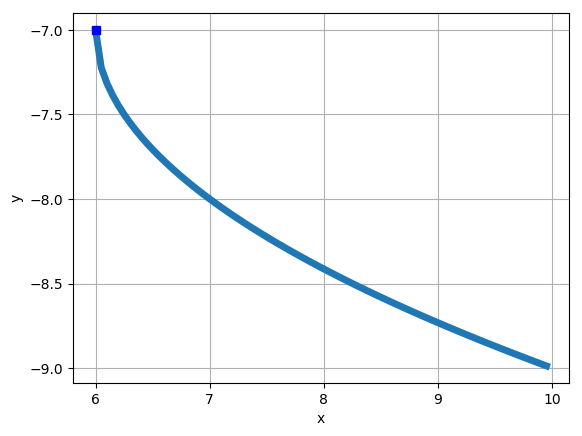
\includegraphics[width=.3\textwidth]{../Figures/question22MU.png}
\end{center}

\columnbreak

	\begin{enumerate}[label=\Alph*.]
		\item $f(x) = \sage{choices[0]}$ 
		\item $f(x) = \sage{choices[1]}$ 
		\item $f(x) = \sage{choices[2]}$ 
		\item $f(x) = \sage{choices[3]}$  
	\end{enumerate}
\end{multicols}
\vspace*{-3mm} 
}
%\pagebreak
% Objective 2 - Identify the graph of a radical function (graph to equation).
\begin{sagesilent}
problemNumber = 23
load("../Code/radical/radicalEquationToGraph.sage")
\end{sagesilent}

\litem{\sage{displayStem}

$$ f(x) = \sage{displayProblem} $$

	\begin{enumerate}[label=\Alph*.]
\begin{multicols}{2}
		\item \begin{center}
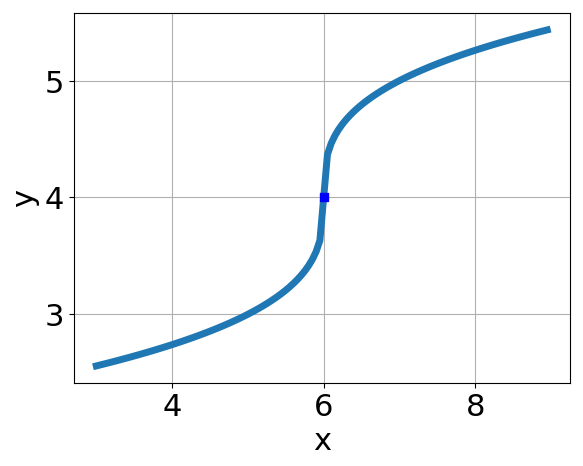
\includegraphics[width=.3\textwidth]{../Figures/question23MUA.png}
\end{center}
		\item \begin{center}
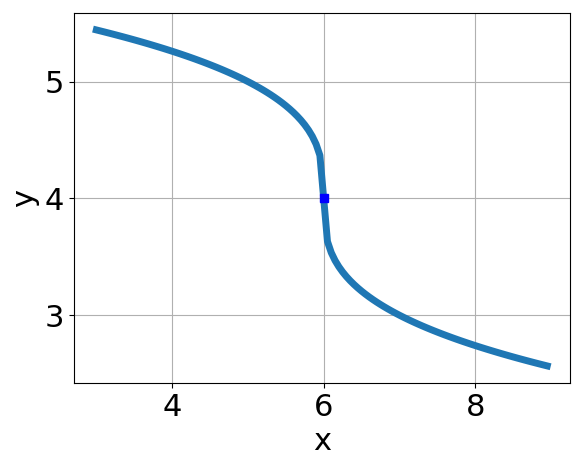
\includegraphics[width=.3\textwidth]{../Figures/question23MUB.png}
\end{center}
\columnbreak
		\item \begin{center}
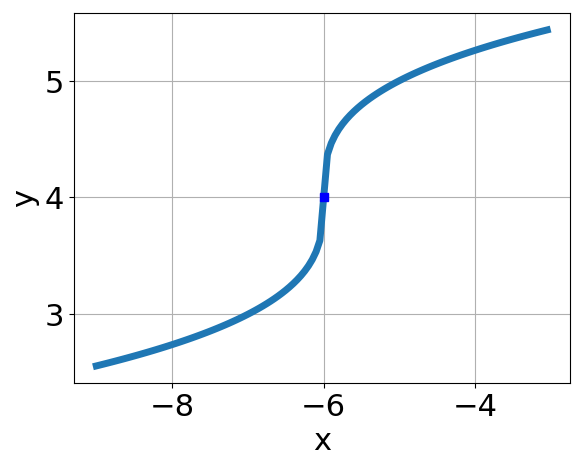
\includegraphics[width=.3\textwidth]{../Figures/question23MUC.png}
\end{center}
		\item \begin{center}
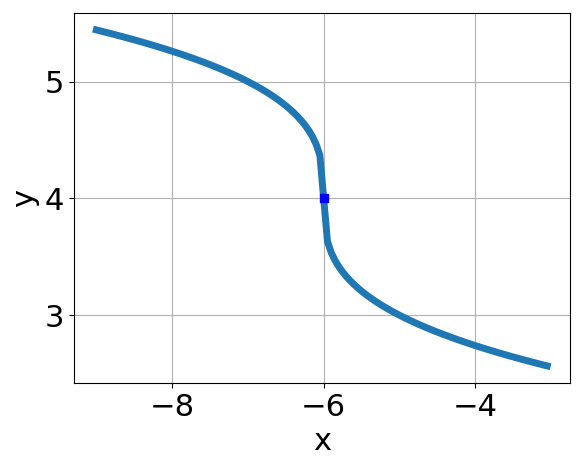
\includegraphics[width=.3\textwidth]{../Figures/question23MUD.png}
\end{center}
\end{multicols}
	\end{enumerate}	
}

% Objective 3 - Solve radical equations that lead to linear equations.
\begin{sagesilent}
problemNumber = 24
load("../Code/radical/solveRadicalLinear.sage")
\end{sagesilent}

\litem{\sage{displayStem}

$$ \sage{displayProblem} $$

	\begin{enumerate}[label=\Alph*.]
		\item $\sage{choices[0]}$ 
		\item $\sage{choices[1]}$ 
		\item $\sage{choices[2]}$ 
		\item $\sage{choices[3]}$  
		\item $\sage{choices[4]}$
	\end{enumerate}	

}

% Objective 4 - Solve radical equations that lead to quadratic equations.
\begin{sagesilent}
problemNumber = 25
load("../Code/radical/solveRadicalQuadratic.sage")
\end{sagesilent}

\litem{\sage{displayStem}

$$ \sage{displayProblem} $$

	\begin{enumerate}[label=\Alph*.]
		\item $\sage{choices[0]}$ 
		\item $\sage{choices[1]}$ 
		\item $\sage{choices[2]}$ 
		\item $\sage{choices[3]}$  
		\item $\sage{choices[4]}$
	\end{enumerate}	

}

\end{enumerate}	

\end{document}